\chapter{SPIN STRUCTURE OF PROTON}

\section{Introduction}

A proton is a complex composite structure comprising three quarks: two up ($u$) and one down ($d$). Most of its spin structure comes from sources other than its valence quarks. After the compelling discovery of the EMC collaboration \cite{EuropeanMuon:1987isl}, understanding the proton structure has become challenging for the particle physicist community. While the proton constituents are well understood, their contribution to the proton spin is still puzzling. Despite tremendous development in the experiment and theory of (non-)perturbative QCD, we are not yet able to fully understand how quarks and gluons spin and orbital angular momentum contribute to the proton's spin. 

The knowledge of the proton spin structure is based on annihilation and scattering experiments. In the annihilation experiments, leptons -antileptons - beams are used. When highly energetic lepton and anti-lepton beams collide, they annihilate to form a highly energetic virtual photon (as leptons undergo electromagnetic interaction) enough to generate a quark and antiquark pair rapidly flying apart. As they fly, they are pulled so strongly to store more energy, and in the vicinity of the proton's radius, they break apart radiating gluons, which further fragment into quark and anti-quark pairs. This is called the fragmentation process. This process continues until the energy is compensated for by producing streams of particles in the form of jets. In the process, (anti-)quarks combine to form a stable colorless state  of baryons and mesons, which is called hadronization. Analyzing the jets or exclusive particles along the direction of the initial parton provides information about the partonic structure of the nucleon. 

On the other hand, the scattering experiments used either lepton-proton collision or proton-proton ($pp$) collision. In both cases, enough energy is supplied in the colliding beams such that a quark in the proton gets knocked out and undergoes fragmentation and hadronization process as in the annihilation process producing jets, which serve as a proxy for the partons producing it.  

%definition of PDFs, TMDs, and GPDs
The proton's parton structure is characterized by a parton distribution function (PDF) and fragmentation functions (FFs). These functions provide insight into the distribution of momentum carried by the partons within the proton. Assuming the probed nucleon is moving along the $\hat{z}$ direction, then the extension of longitudinal momentum-dependent PDF can be made in the momentum space or in the coordinate space. The transverse momentum extension to the longitudinal momentum dependence PDF is called the transverse momentum dependent PDFs\cite{Collins:1981uw, Mulders:1995dh, Boer:1997nt, Bacchetta:2006tn}, whereas the extension in the coordinate space is called the generalized parton distributions (GPDs)\cite{Ji:1996ek, Muller:1994ses, Radyushkin:1997ki}. The longitudinal momentum-dependent PDFs, TMDs, and GPDs enable three-dimensional tomography of the proton structure. These distributions not only describe the parton composition within the proton but also links the parton properties from the  strong QCD interactions to the nucleon. 

\section{Leading Twist Transverse Momentum Dependent Distribution Functions}
The PDFs depend on the polarization state of the nucleon and the parton within the nucleon. There exist eight leading-order TMD, whose physical description is listed in Figure \ref{fig:tmdpdfs}. $f_1(x, k_T)$ is the simplest unpolarized TMD, which describes a probability of finding a quark carrying longitudinal momentum $x$ of the nucleon and a transverse momentum $k_T=|\vec{k}_T|$ in a fast-moving nucleon. For an unpolarized nucleon, the transverse quark distribution is given by the Boer-Mulder function, $h_{1}^\perp(x, k_T)$.  If the nucleon is polarized longitudinally to the momentum direction, then the longitudinal quark distribution is given by the helicity PDF $g_{1L}(x, k_T)$ and a transverse distribution is given by Worm Gear $h_{1L}(x, k_T)$. The Sivers function, $f_{1T}^\perp(x, k_T)$, is introduced to describe spin-independent quark distribution in a transversely polarized nucleon. Furthermore, for a transversely polarized nucleon, the longitudinal quark polarization is given by a Worm Gear, $g_{1T}(x, k_T)$, and a transverse quark polarization is given by transversity $h_{1T}(x, k_T)$ or the pretzolosity $h_{1T}^\perp(x, k_T)$. The Sivers, Boer-Mulders, and pretzelosity require orbital angular momentum in the nucleon since they involve a transition between initial and final nucleon states whose orbital angular momentum differs by $\pm 1$ (Sivers and Boer-Moulder) or by $\pm 2$ (pretzelosity). The Worm-gears link two perpendicular spin directions and are also connected to the quark orbital motion inside nucleons \cite{Aidala:2012mv}.

\begin{figure}[H]
    \centering
    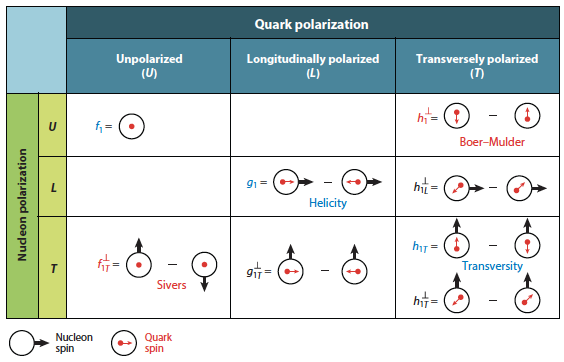
\includegraphics[scale=0.6]{MisImages/Ch2Images/pdfs.png}
    \caption{Leading twist TMDs classified according to the quark polarizations (f, g, h) and nucleon (U, L, T) \cite{Accardi:2012qut}. A similar classification of TMD distributions exists for gluons.}
    \label{fig:tmdpdfs}
\end{figure}
    
The three TMD distributions: $f_1(x, k_T)$, $g_{1L}(x, k_T)$, and $h_{1T}(x, k_T)$, survives upon integration over the $k_T$ as they are even under the exchange of $k_T\rightarrow -k_T$, leading to three collinear PDFs. All the other TMD distributions are $k_T-$odd, which vanishes upon $k_T$ integration. These $k_T-$odd TMDs are beyond the scope of this thesis; Only the leading order TMD distribution functions will be discussed, focusing on the transversity PDF.   

The quest for transverse spin provides a unique way to unravel the proton spin structure. The spin of the proton perpendicular to the proton's momentum direction is a vector that correlates with the transverse component of the parton (TMD) or the transverse position of the parton (GPD). The first observation of the single spin asymmetry (SSA) was in 1976 from  polarized $pp$ data at $\sqrt{s}$=6 GeV and 12 GeV for the charged pions at Argonne National Laboratory Zero Gradient Synchroton \cite{Klem:1976ui}. This observation was supported by similar experiments \cite{Dragoset:1978gg, Antille:1980th, Apokin:1990ik, Saroff:1989gn}. Similar asymmetries have been observed in polarized $pp$ by the RHIC where the asymmetry reaches up to 40\% \cite{Aschenauer:2016our}, lepton-nucleon experiment in at HERMES, COMPASS, and JLab. The observed asymmetry in the hadron production off the polarized nucleon tells us about the spin-orbit coupling in the nucleon and/or in the fragmentation process \cite{Aidala:2012mv}.    

The quantitative understanding of PDFs has been achieved through QCD analysis of an extensive dataset, encompassing experiments such as Deep Inelastic Scattering (DIS), Drell-Yan lepto-production, and inclusive processes in $pp$ collisions \cite{pdfCTEQ:2021, DSSV:2019, Cocuzza:2023oam}.
At the leading twist, the nucleon structure is fully described by three Parton Distribution Functions (PDFs): the unpolarized PDF, $f_1(x)$, the helicity PDF, $g_1(x)$,  and the transversity PDF, $h^q_1(x)$, where $x$ is the nucleon momentum fraction carried by patrons. Although $f_1(x) $ and $g_{1}(x)$ are reasonably well constrained by experimental data \cite{EurPhys,deFlorian:2009vb}, the knowledge of $h_1^{q}(x)$ is limited \cite{Anselmino:2013vqa, Kang:2015msa, Radici:2018iag} to semi-inclusive deep inelastic scattering (SIDIS) \cite{HERMES:2008mcr, HERMES:2009lmz, COMPASS:2008isr, COMPASS:2012bfl, COMPASS:2014bze, JeffersonLabHallA:2011ayy}, $e^+e^-$ \cite{BaBar:2013jdt, Belle:2008fdv} and $p^\uparrow p$ \cite{STAR:2015jkc} data. This is because $h_1^{q}(x)$ is a chiral-odd object, and it needs to be coupled with another chiral-odd partner to form a chiral-even cross section that is experimentally observable.

\section{Current Understanding of the Collinear PDFs}
\subsection{Unpoalrized PDF}
Unpolarized PDF, $f_1(x)$, describes the probability of finding an unpolarized parton within an unpolarized proton as a function. $f_1(x)$ is well constrained by the global QCD analysis of a vast amount of experimental data from the ATLAS, CMS, and LHCb data from the Large Hadron Collider (LHC), HERA I+II combined DIS data, and measurements from the fixed-target data from Fermilab Tevatron $p\bar{p}$ collider by CTEQ \cite{Dulat:2015mca, pdfCTEQ:2021}, MSHT \cite{Harland-Lang:2014zoa, Bailey:2020ooq}, and NNPDF \cite{NNPDF:2017mvq} groups. Figure \ref{fig:cteqpdf} shows the most recent global QCD analysis of $f_1(x)$ as a function of $x$ for the different quark flavors and the gluon from CTEQ collaboration. The higher $x$ region is dominated by the valence quarks, $u$ and $d$, and gluons. The $f_1(x)$ for gluon is scaled down by the factor of 5, and it indicates that the gluons contribute as much as the valence quarks in the valence region and completely dominate in the lower $x$ region. Although the high$-x$ region is well constrained ($0.1<x$), the low-$x$ region is not well understood, which requires much higher center-of-mass energy collision data, and very limited experimental data is available to probe in this region. 
\begin{figure}[H]
    \centering
    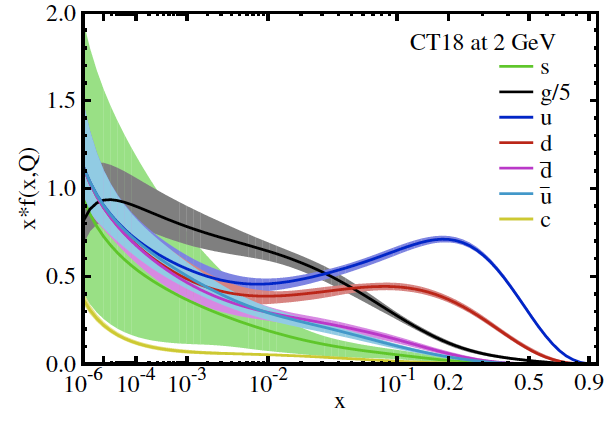
\includegraphics[scale=0.5]{MisImages/Ch2Images/pdfsCT18_fx2GeV.png}
    \caption{Unpolarized PDFs at $Q$ = 2 GeV for $u$, $\bar{u}$, $d$, $\bar{d}$, $s=\bar{s}$, and $g$. The gluon PDF has been scaled down as $g(x, Q)$/5 \cite{pdfCTEQ:2021}.}
    \label{fig:cteqpdf}
\end{figure}

\subsection{Helicity PDF}
The helicity PDF, $g_1(x)$, is defined as the probability of finding a longitudinally polarized parton in a longitudinally polarized nucleon. The $g_1(x)$ for the quarks are mainly constrained by the DIS data. However, the DIS data are less sensitive to the gluons, and polarized $pp$ collision data from RHIC is crucial to probe the gluon polarization. The first evidence of the gluon polarization is established by the global QCD analysis from DSSV14 \cite{DSSV:2014} and confirmed by NNPDF \cite{NNPDF:2017mvq}, and further constrained by DSSV14 \cite{DSSV:2019} utilizing the di-jet measurements from the RHIC \cite{STARdijet:2016, STARdijet:2018}.

Figure \ref{fig:dssv_quark} shows the $g_1(x)$ from DSSV14 for different quark and antiquark flavors, compared to the NNPDFpol1.1. The $u-$quark has a positive helicity, and $d-$quark has negative helicity, meaning that the $u-$quark tends to align its spin along the nucleon polarization, whereas the $d-$quark tends anti-align to the nucleon spin. Helicity PDF for quarks is approaching the precision of the unpolarized. However, the gluon helicity is far from reach to the quark precision level, which is shown in Figure \ref{fig:dssv_gluon}. 
\begin{figure}[H]
    \centering
    \begin{subfigure}{1\textwidth}
    \centering
    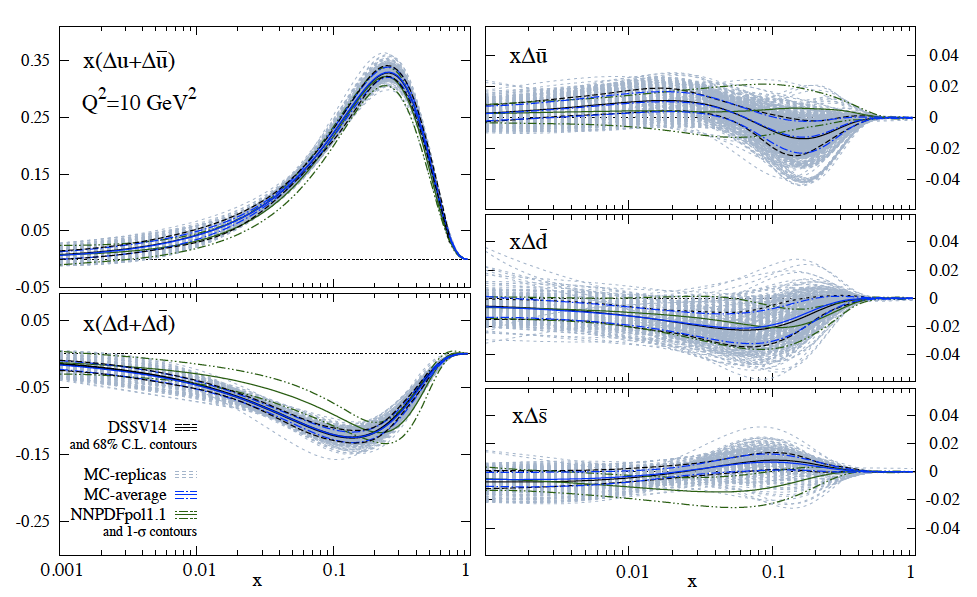
\includegraphics[scale=0.4]{MisImages/Ch2Images/pdfDSSV_gxQ.png}
    \subcaption{Helicity PDFs for the quark and antiquark at $Q^2$ = 10 $\mathrm{GeV^2}$.}
    \label{fig:dssv_quark}
    \end{subfigure}
    \begin{subfigure}{1\textwidth}
    \centering
    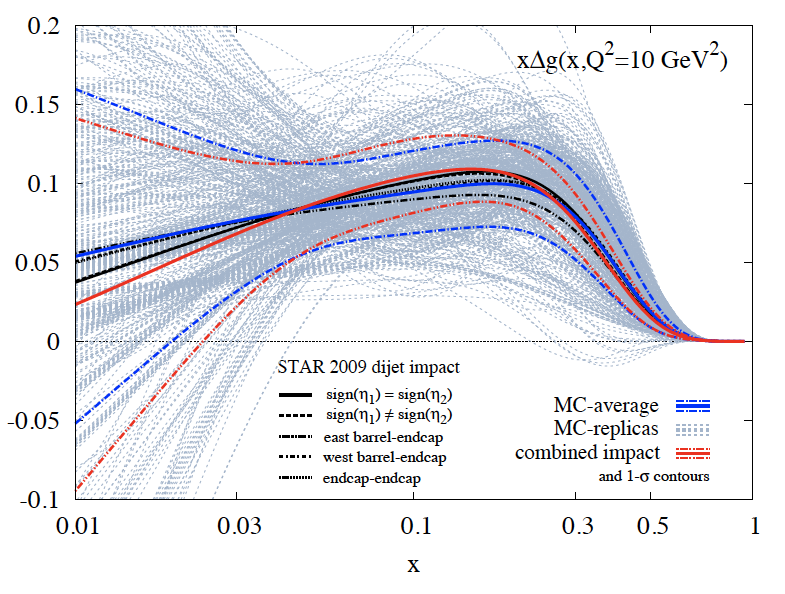
\includegraphics[scale=0.5]{MisImages/Ch2Images/pdfDSSV_gxG.png}
    \subcaption{ Gluon helicity distribution.}
    \label{fig:dssv_gluon}
    \end{subfigure}
    \caption{Helicity PDF for gluon.}
\end{figure}

\subsection{Transversity PDF}
At the leading twist, transversity PDF ($h_1^q(x)$) is defined as the probability of finding a transversely polarized quark in a transversely polarized nucleon, which was first introduced by Ralston and Soper \cite{Ralston:1979}. $h_1^q(x)$  is only a valence quark property and vanishes for the gluon \cite{Barone:2001}. Current understanding of $h_1(x)$ is from global analysis of the SIDIS data from the HERMES \cite{HERMES:2004, HERMES:2008mcr, HERMES:2010} and COMPASS \cite{COMPASS:2008isr, COMPASS:2012bfl, COMPASS:2014bze}, $e^+e^-$ data from Belle \cite{Belle:2008fdv, Belle:2011, Belle:2017} and BABAR\cite{BaBar:2013jdt}, and $pp$ data from STAR \cite{STAR:2015jkc, STAR:2017wsi}. The phenomenological extraction of $h_1(x)$ from these data can be found in Ref. \cite{Kang:2015msa, Radici:2018iag, Cocuzza:2023oam}. 



\begin{figure}[H]
    \centering    
    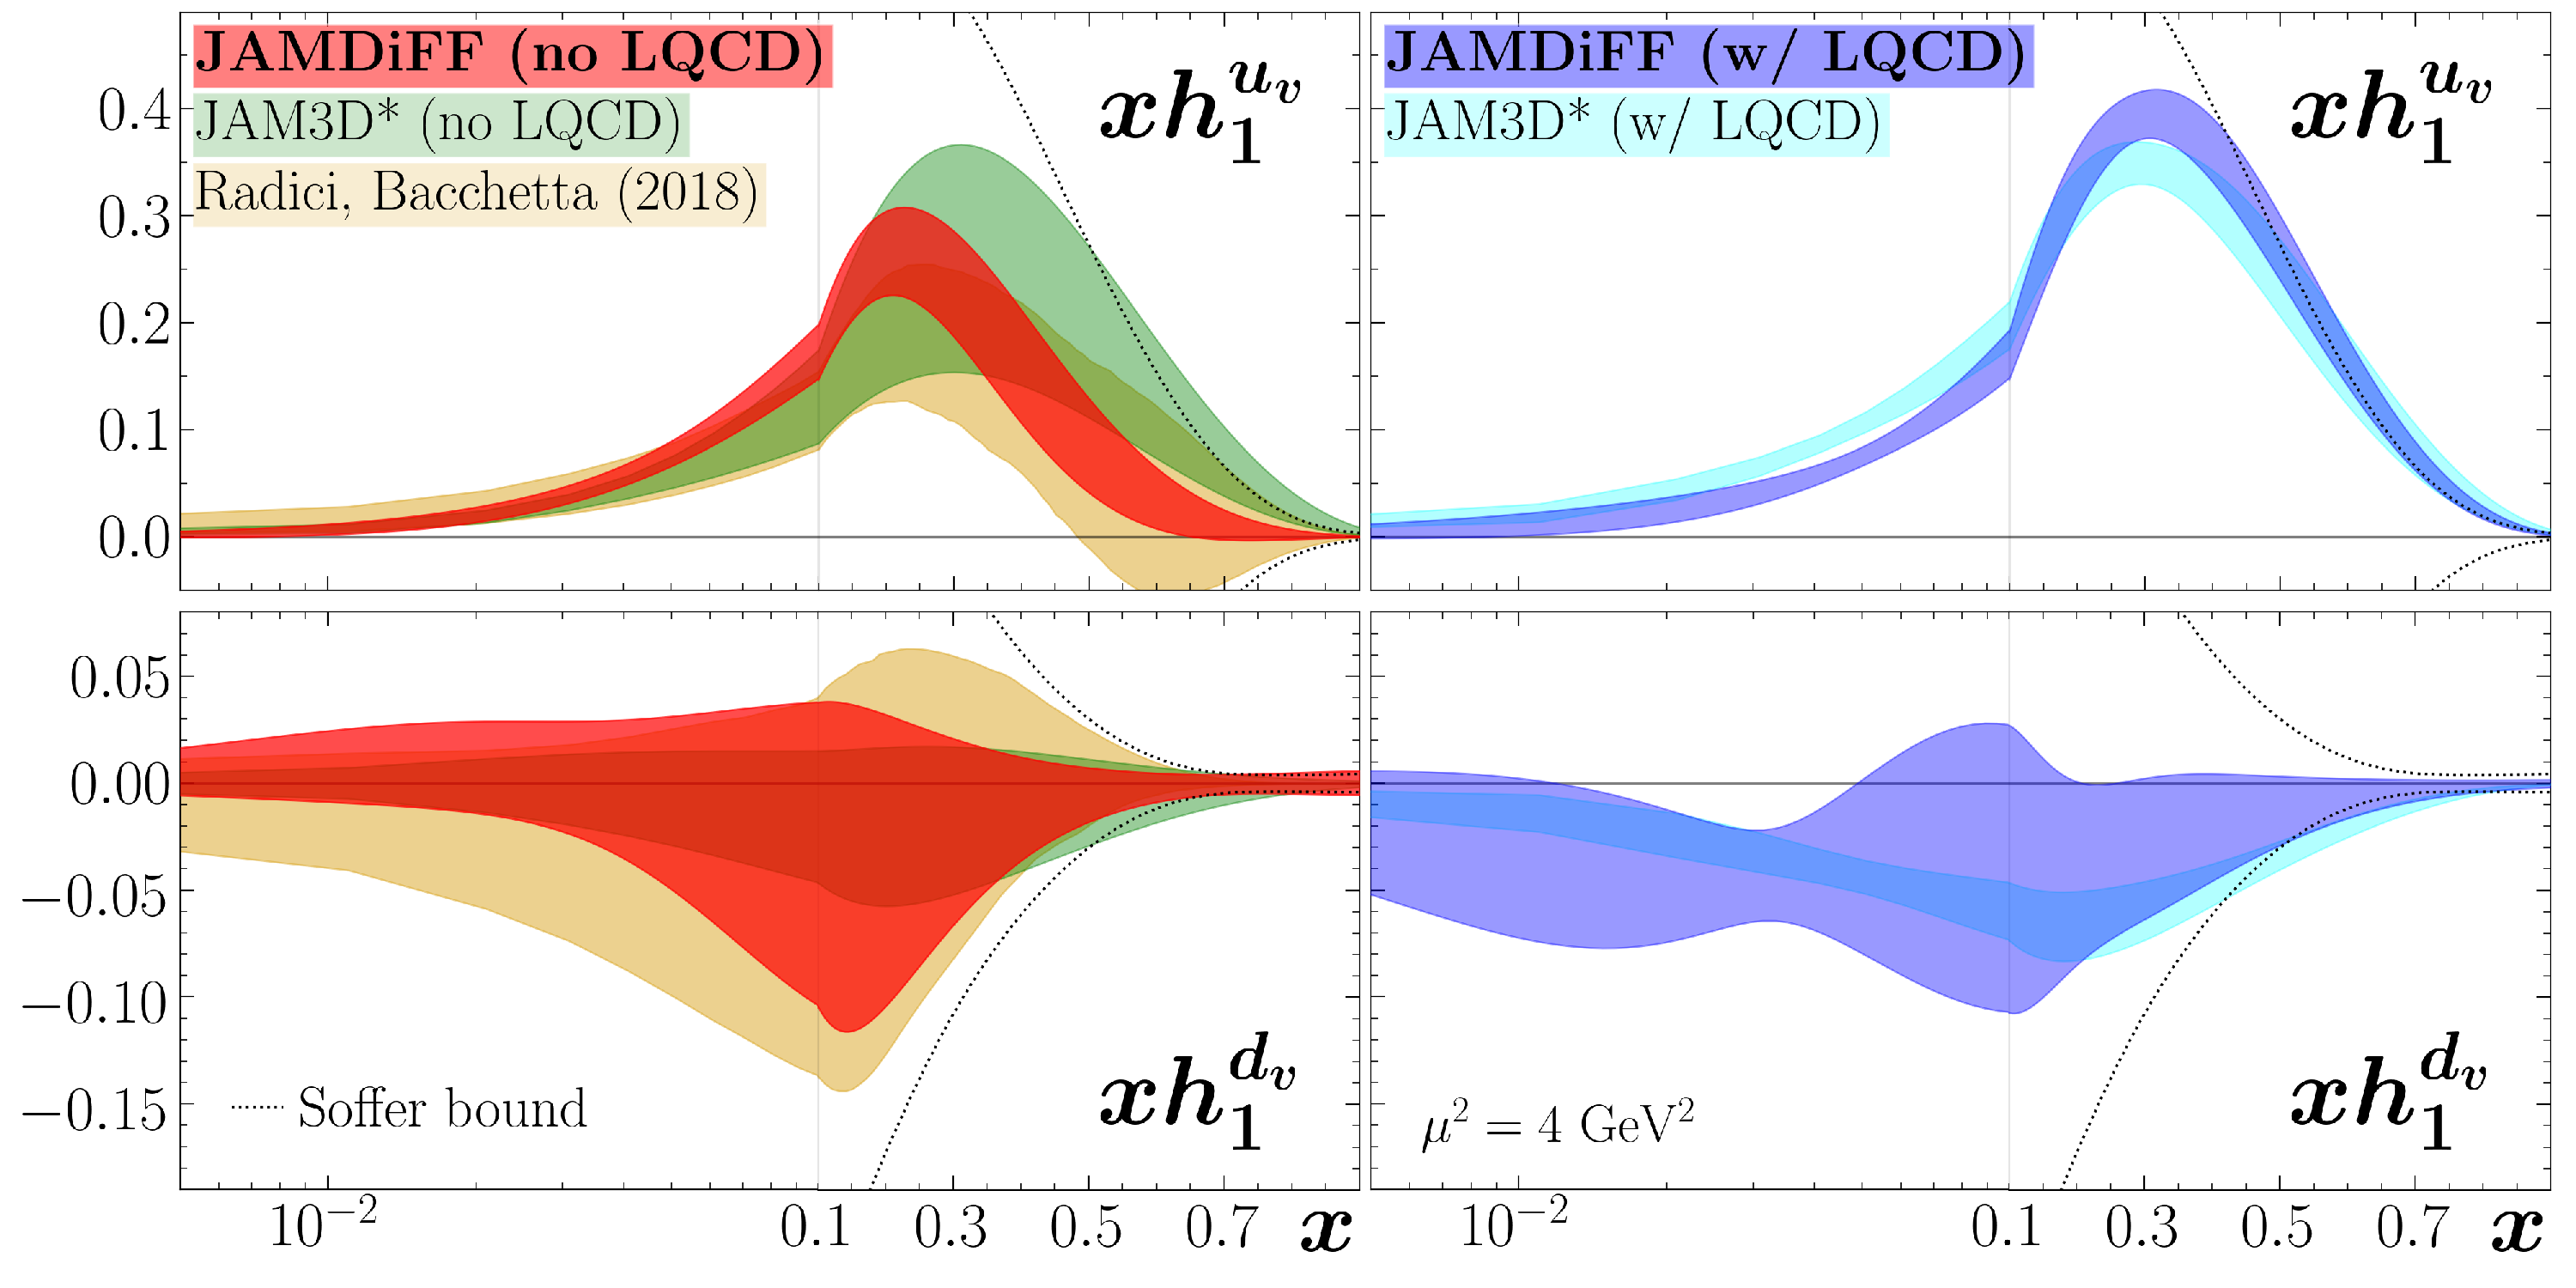
\includegraphics[scale=0.3]{MisImages/Ch2Images/pdfJAM_h1.pdf}
    \caption{Transversity PDF from the JAM collaboration.}
    \label{fig:jamtrans}
\end{figure}

Figure \ref{fig:jamtrans} depicts the recent global extraction of $h_1(x)$ from JAM collaboration \cite{Cocuzza:2023oam}, compared to the extraction from Ref. \cite{Radici:2018iag} (left panel) including the lattice QCD data (right panel) \cite{Gupta:2018, Hasan:2019}. The $h_1(x)$ for the valence quarks feature a similar trend as the $g_1(x)$ but unconstrained by far, even in the valence quark region. The inclusion of the LQCD data, however, appears to constrain significantly.    

\section{Fragmentation Functions}
Fragmentation functions (FFs)  usually appear as a non-perturbative ingredient in the factorization formula when the specific particle species are observed in the final state. FF is defined as the probability of finding  color-neutral particles inside partons. In other words, it describes how color-neutral particles are formed from the colored quarks and gluons.

FF can be studied in single-inclusive hadron production in $e^+e^-$ (SIA), in SIDIS and $pp$ collision processes, where FF frequently appears in the QCD factorized cross section: 
\begin{itemize}
    \item SIA: $\sigma^{e^+e^- \rightarrow hX} = \hat{\sigma}\otimes FF$
    \item SIDIS: $\sigma^{lN \rightarrow lhX} = \hat{\sigma}\otimes PDF \otimes FF$
    \item $pp$: $\sigma^{pp \rightarrow hX} = \hat{\sigma}\otimes PDF \otimes PDF \otimes FF$
\end{itemize}
where $\hat{\sigma}$ represents the process-dependent hard scattering cross section, which is perturbatively calculable, and only the leading order factors are shown. This factorization scheme holds true only if the hard scale is present in each of the processes, such as the center-of-mass energy, $\sqrt{s}$, serves as a hard scale in the SIA, the virtual momentum transfer between lepton and hadron, $Q^2$, serves as a hard scale on the SIDIS, and the transverse momentum of the final state hadron relative to the proton's momentum, $p_{h\perp}$, serves as a hard scale. 

The application of FF was first introduced in the 1970s to explain the observation of large transverse momentum of hadrons in the hadronic collisions from CERN, which could not be explained without including gluonic subprocesses \cite{Metz:2016}. Several FFs appear in the process depending on the inclusion of spin of the hadron and/or parton, transverse momentum of hadron relative to the parton, higher-twist effects, and fragmentation to more than one hadrons, which are summarized in Table \ref{tab:ffs}. 

%TMD fragmentation functions table
\begin{table}[H]
    \centering
    \begin{tabular}{|c|c|c|c|}
    \hline
   \diagbox{H}{q(g)} & U & L (Circ) & T (Lin)  \\
   \hline
    U & $D_1^{h/q(g)}$ & & $H_1^{\perp h/q(g)}$ \\
    \hline
    L &  & $G_1^{h/q(g)}$& $H_{1L}^{\perp h/q(g)}$  \\
    \hline  
    T & $D_{1T}^{\perp h/q(g)}$ & $G_{1T}^{h/q(g)}$ & $H_1^{h/q(g)}$ $H_{1T}^{\perp h/q(g)}$  \\
    \hline     
    \end{tabular}
    \caption{Interpretation of TMD FF for quarks (gluons). }
    \label{tab:ffs}
\end{table}

The $D_1^{h/q(g)}$ is the unpolarized FF, which describes the number density of unpolarized hadrons in an unpolarized quark (gluon). The density of longitudinally polarized hadrons in longitudinally(circularly) polarized quark(gluon) is given by $G_1^{h/q(g)}$. The $H_1^{h/q(g)}$ describes the density of transversely polarized hadron in transversely (linearly) polarized quark(gluon). One should remember that if the parton polarization is involved, then the FF gives the difference in densities, such as $D_1^{h/q(g)}$ has a simple number density interpretation; however, $G_1^{h/q(g)}$ represents the difference in densities of two opposite parton polarization. $H_1^{\perp h}$ is well-known Collins FF \cite{Collins:1992kk}, as it provides access to the transversity in the SIDIS process.


The dihadron FFs (DiFFs) appear in the factorization formula of the processes, where a parton fragments in two hadrons. It is gaining more attention lately because it can be an analyzer for the transversity in the collinear framework, unlike the TMD Collins FF. The DiFFs measure the probability of finding two color-neutral hadrons in a parton. $D_1^{h_1h_2}$ represents the measure of such probability for two hadrons $h_1$ and $h_2$ in an unpolarized parton. Including the transverse momentum of parton $k_T$ and the polarization, the probability density of finding two unpolarized hadrons  in a transversely polarized target is given by two DiFFs: $H_1^{\sphericalangle, h_1h_2}$ and $H_1^{\perp, h_1h_2}$ \cite{Metz:2016}. The $H_1^{\sphericalangle, h_1h_2}$ is a well-studied DiFF than other DiFFs, as it provides access to the transversity, for example, in polarized $pp$ collisions. It is often called the Interference Fragmentation Function (IFF) because it requires interference between different dihadron production channels for its survival \cite{Jaffe:1997hf, Jaffe:1997pv, Bacchetta:2004it}.       

\section{Accessing Transversity Via Dihadron Channel: Theoretical Description}
\label{sec:ifftheory}
 Accessing the transversity PDF, which is chiral-odd, can be quite challenging. This must be combined with another chiral-odd partner to yield a chiral-even cross-section. As a result, it cannot be accessed in inclusive processes. Furthermore, to access transversity, knowledge of another chiral-odd object that needs to appear together is required. This difficulty makes it less straightforward to access than other leading-order parton distribution functions, making it the least understood among other leading-order PDFs.

Transversity can be accessed through a single hadron production, either by exploiting TMD factorization (e.g., Collins effect \cite{Collins:1992} in SIDIS) or collinear sub-leading twist (twist 3) factorization in hadronic collisions \cite{DAlesio:2020vtw, Cammarota:2020qcw}.
 Alternatively, one can consider the unpolarized dihadron production at leading twist collinear factorization, where transversity couples with the interference fragmentation function, $H^\sphericalangle_1$ (IFF) \cite{Tang:1998wp, Jaffe:1997hf, Jaffe:1997pv, Bacchetta:2004it}.
 The collinearity is preserved in this channel as the dihadron center of mass travels along the jet axis, and the IFF survives even after integrating over the transverse momentum of the hadron pair. Moreover, this channel doesn't require a jet reconstruction, devoid of systematic uncertainty associated with the jet reconstruction.  

The discussion will focus solely on accessing transversity through the dihadron channel in $p^\uparrow p$ collision. This specific channel is used to measure the azimuthal correlation asymmetry in this analysis, which can be expressed as,
\begin{equation}
    \label{eq:dihadch}
    p^\uparrow_a(\mathbf{S_a, P_a}) + p_b (\mathbf{P_b}) \rightarrow (h_1 h_2)_{jet} (\mathbf{P_h})  + X,
\end{equation}
where $p^\uparrow_a(p_b)$ is a transversely polarized (unpolarized) proton, $h_1$ and $h_2$ are the final state unpolarized charged hadrons  within a jet, and $X$ represent undetected final state particles. The boldface quantities in the equation are regular three vectors, where $\mathbf{S}$ is the polarization vector and $\mathbf{P}$ is the momentum vector. The final state hadrons could be protons, kaons, or pions.

\drawgraphics{0.8}{Results/IFF2015/ppcol.png}{Dihadron channel in $p^\uparrow p$ showing the fragmentation of polarized parton and final state unpolarized dihadron pair. The respective PDFs and FFs are indicated at where they appear in the process.}{fig:ppcol}

The dihadron channel is depicted schematically in Figure \ref{fig:ppcol}. The polarized (unpolarized) proton originates from the left (right), and the associated kinematic variables are indicated with subscripts $a(b)$. The transversity PDF of a transversely polarized proton $a$ is denoted by $h_1$, while the unpolarized PDF of proton $b$ is denoted by $f_1$. The hard scattering occurs between a transversely polarized parton $i$ from proton $a$ and an unpolarized parton $j$ from proton $b$. The cross section of the hard scattering, denoted as $\hat{\sigma}$, is perturbatively calculable. This scattering occurs at an extremely small distance ($\lesssim 10^{-15}$ m), where the partons are considered asymptotically free. Subsequently, the hard scattered partons undergo fragmentation and hadronizes into color-neutral stable particles. The fragmentation of the polarized scattered parton $k$ is described by the spin-dependent fragmentation function $H^\sphericalangle_1$, while the fragmentation of the unpolarized parton $l$ is described by $D_1$. At the leading twist, these fragmentation functions also possess a probabilistic interpretation, representing the probability of finding color-neutral hadrons within the parton. In the final state, we observe hadrons emerging from the polarized parton $k$, either in the form of jets or exclusively, which grants access to the quark transversity coupled with the IFF.

Measuring two hadrons in the final state provides two vectors associated with the hadron pair, offering a convenient theoretical framework \cite{Bacchetta:2003vn}. If $\mathbf{P_{h_1}}$ and $\mathbf{P_{h_2}}$ represent the momenta of the two hadrons, these vectors can be defined as follows:

\begin{equation}
\mathbf{P_h} = \mathbf{P_{h_1}} + \mathbf{P_{h_2}},\ \mathrm{and}\ \mathbf{R} = \mathbf{\frac{P_{h_1} - P_{h_2}}{2}},
\end{equation}

Here, $\mathbf{P_h}$ denotes the resultant momentum of the hadrons, and $\mathbf{R}$ represents the relative momentum vector. Due to the presence of the relative momentum vector $\mathbf{R}$, the IFF can be integrated over the transverse component of $\mathbf{P_h}$ with respect to the jet axis. Additionally, the transverse component of the fragmenting quark can be expressed in terms of the transverse component of the relative momentum, denoted as $\mathbf{R_T}$, through the mixed product $\mathbf{S \cdot R \times P_h}$. In this channel, the center of mass of the hadron pair moves collinearly with the jet axis, thereby preserving the concept of collinear factorization; hence the jet reconstruction is not required.
For a dihadron channel given by equation \ref{eq:dihadch}, only one type of asymmetry, $A_{UT}$,  exists, which is given by, 
    \begin{equation}
        \label{eq:asymxsec}
        A_{UT} = \frac{d\sigma^\uparrow - d \sigma^\downarrow}{d\sigma^\uparrow + d \sigma^\downarrow} \equiv \frac{d\sigma_{UT}}{d\sigma_{UU}},
    \end{equation}
where $d\sigma_{UT}$ is the difference between the cross section when the polarized proton $a$ is polarized up ($\uparrow$) and down ($\downarrow$), whereas $d\sigma_{UU}$ is the unpolarized cross section. The polarized and unpolarized part of the cross section can be expressed as \cite{Bacchetta:2004it}, 

\begin{align}
\label{eq:xsecut}
    d\sigma_{UT} &= 2|\mathbf{P_{h\perp}}|\sum_{i,j,k,l} |\mathbf{S_a}|\ sin(\phi_S - \phi_R)  \int \frac{dx_a dx_b}{8\pi^2 z_h} f_1^{j/b}(x_b)\ h_1^{i/a}(x_a)\ \frac{d\Delta\sigma^{i^\uparrow j \rightarrow k^\uparrow l}}{d\hat{t}} \nonumber \\
     & \times \frac{\mathbf{R}}{M_h}\ sin\theta \ H_1^{\sphericalangle,h_1h_2/k}(z_h, cos\theta, M_h^2)
\end{align}
\begin{align}
\label{eq:xsecuu}
    d\sigma_{UU} &= 2|\mathbf{P_{h\perp}}|\sum_{i,j,k,l} \int \frac{dx_a dx_b}{8\pi^2 z_h} f_1^{i/a}(x_a)\ f_1^{j/b}(x_b)\ \frac{d\Delta\sigma^{ij \rightarrow kl}}{d\hat{t}} \times  D_1^{h_1h_2/l}(z_h, cos\theta, M_h^2)
\end{align}
In the equations above, $|\mathbf{P_{h\perp}}|$ represents the magnitude of the transverse component of $\mathbf{P_h}$ with respect to the beam direction. This component serves as a hard scale for the process. The PDFs $f_1$ and $h_1$ correspond to the unpolarized and transversity PDFs, respectively. $H_1^{\sphericalangle h_1h_2}$ denotes the IFF, while $D_1^{h_1h_2}$ represents the unpolarized counterpart of the IFF.

The definitions of the azimuthal angles $\phi_S$ and $\phi_R$ are derived from Figure \ref{fig:angles} and are given by Equations \ref{eq:cosang}-\ref{eq:sinang}. These angles are defined in the center of mass of the hadronic system. Specifically, $\phi_S$ denotes the angle between the scattering plane formed by $\mathbf{P_a}$ and $\mathbf{P_h}$, and the polarization vector $\mathbf{S_a}$. On the other hand, $\phi_R$ represents the angle between the scattering plane and the dihadron plane formed by the momenta $\mathbf{p_{h_1}}$ and $\mathbf{p_{h_2}}$.

The hard scale is assumed to exceed the dihadron system's proton mass significantly and the invariant mass, denoted as $M_h$. The validity of the assumptions holds only at the leading twist (leading order in $1/|\mathbf{P_{h\perp}}|$).
\begin{equation}
    \label{eq:cosang}
    cos \phi_S = \frac{\hat{P_a}\times \mathbf{P_h}}{|\hat{P_a}\times \mathbf{P_h}|}\cdot \frac{\hat{P_a}\times \mathbf{S_a}}{|\hat{P_a}\times \mathbf{S_a}|}, \hspace{2em}     cos \phi_R = \frac{\hat{P_h}\times \mathbf{P_a}}{|\hat{P_h}\times \mathbf{P_a}|}\cdot \frac{\hat{P_h}\times \mathbf{R}}{|\hat{P_h}\times \mathbf{R}|} 
\end{equation}
\begin{equation}
    \label{eq:sinang}
sin \phi_S = \frac{(\mathbf{P_h}\times \mathbf{S_a})\cdot \hat{P_a}}{|\hat{P_a}\times \mathbf{P_h}||\hat{P_a}\times \mathbf{S_a}|}, \hspace{2em} sin \phi_R = \frac{(\mathbf{P_a}\times \mathbf{R})\cdot \hat{P_h}}{|\hat{P_h}\times \mathbf{P_a}||\hat{P_h}\times \mathbf{R}|}
\end{equation}

The polarized cross section exhibits a sinusoidal modulation of the azimuthal angle $\phi_{RS}$ (defined as $\phi_S - \phi_R$), while such modulation is suppressed in the unpolarized cross section. This observation indicates a bias in the dihadron yields within the specific $\phi_{RS}$ bin, resulting in an asymmetry that arises solely from polarization effects. By utilizing Equations \ref{eq:xsecut} and \ref{eq:xsecuu}, Equation \ref{eq:asymxsec} can be expressed as follows:

\begin{equation}
A_{UT}^{sin\phi_{RS}} = \frac{1}{|\mathbf{S_a}|}\frac{d\sigma^\uparrow - d\sigma^\downarrow}{d\sigma^\uparrow + d\sigma^\downarrow},
\end{equation}

This equation isolates $A_{UT}$ as the amplitude of the "sine" modulation of dihadron yields in $\phi_{RS}$ at the leading twist. To represent the asymmetry associated with the "sine" modulation in $\phi_{RS}$, it will henceforth be denoted as \aut. Experimental measurement of \aut\ involves counting the number of dihadrons in $\phi_{RS}$ bins for both beam polarizations ($\uparrow$ and $\downarrow$), which is sensitive to the product $h_1 H^\sphericalangle_1$:

\begin{equation}
A_{UT} \propto \sum_{i,j,k,l} \frac{f_1^{j/b}(x_b) h_1^{i/a}(x_a) H_1^{\sphericalangle h_1h_2/k}(z_h,M^2_h) }{f_1^{j/b}(x_b) f_1^{i/a}(x_a) D_1^{h_1h_2/l}(z_h, M^2_h)},
\end{equation}

Here, all components are non-perturbative objects, and precise experimental knowledge is required to extract transversity. The unpolarized PDF is known to have higher precision based on SIDIS data \cite{H1:2015ubc}, and the IFF has limited knowledge from the $e^+e^-$ experiments. However, the unpolarized Fragmentation Function (FF) $D_1^{h_1h_2}$ lacks experimental constraints, and the global extraction of transversity relies on simulations, leading to large model-dependent uncertainties. To constrain $D_1$ and, consequently, transversity, it is crucial to experimentally measure $d\sigma_{UU}$, an observable discussed in Chapter \ref{chapter:xsec} that is of great importance.

\drawgraphics{0.7}{ImgIFF/geom.png}{The azimuthal angle definitions in the dihadron channel.}{fig:angles}

The relative partial wave expansion of FFs in the  cross sections $d\sigma _{UT}$ and $d\sigma_{UU}$ using the basis of Legendre polynomials through the cos$\theta$ dependence provides intriguing physics insight \cite{Bacchetta:2002ux}. Keeping up to $L=1$, we have,
\begin{equation}
D_1(z, cos\theta, M^2_h)\rightarrow D_{1,oo}(z,M_h^2)+ D_{1,ol}(z,M_h^2) cons\theta + D_{1,ll}(z,M_h^2)\frac{1}{4}(cos^2\theta -1)
\end{equation}
\begin{equation}
sin\theta H_1^\sphericalangle(z, cos\theta, M^2_h)\rightarrow H_{1,ot}^\sphericalangle(z, M^2_h)sin\theta+ H_{1,lt}^\sphericalangle(z, M^2_h)sin\theta cos\theta
\end{equation}
In this context, the double-index notation is used to describe the polarization state in the center of mass of the dihadron for each specific probability amplitude. For instance, $D_{1, oo}$ corresponds to the decay into a $L=0$ pair (s-wave), while $D_{1,ol}$ refers to the interference between the decay amplitudes of a $L=0$ pair and a $L=1$ pair (s-p interference) polarized longitudinally along the center of mass of $\mathbf{P_h}$. Similarly, $H_{1,ot}^\sphericalangle$ represents the interference between the decay amplitudes of a $L=0$ pair and a transversely polarized $L=1$ pair. Furthermore, $H_{1, lt}$ and $D_{1, ll}$ denote the interference between decay amplitudes at different polarization states of $L=1$ pairs.

The $p$-wave contribution arises from the spin-1 resonance in the dihadron production channel. As a result, the $p$-wave fragmentation functions (FFs) ($ll$ or $lt$ terms) exhibit a characteristic mass dependence, with a distinct resonance peak around the mass of the $\rho$ meson ($\sim 0.77$ GeV/$c^2$). On the other hand, the interference terms ($ol$ or $ot$ terms) require the presence of both $s$- and $p$-wave channels. Therefore, the intrinsic FFs are expected to be significant near the $\rho$ meson mass region \cite{Jaffe:1997hf, Bacchetta:2002ux, Bacchetta:2004it}.

\section{Experimental Data for DiFFs}
From the discussion in \ref{sec:ifftheory}, it is clear that independent measurement of $H_1^{\sphericalangle h_1h_2}$
and $D_1^{h_1h_2}$ with $z$ and $M_h$ dependence is required to decouple transversity from the $h_1H_1^\sphericalangle$. 

The recent Belle measurements of $\pi^+\pi^-$ cross section differential in $M_h$ and $z$ \cite{Belle:2017} provide crucial observable for the $D_1^{h_1h_2}$ for quarks. However, these measurements are less sensitive to gluon fragmentation. The measurement from the $pp$ data is required to probe gluon fragmentation. 
The unpolarized $\pi^+\pi^-$ cross section measurement in $pp$ collision data from the STAR experiment (Chapter \ref{chapter:xsec}) will fulfill the dire need of this observable for the first time. Belle also measured back-to-back dihadron single spin asymmetry (SSA) sensitive to the spin-dependent IFF \cite{Belle:2011}. The measured SSA is proportional to the product $H_1^\sphericalangle \bar{H_1^\sphericalangle}$. 

The SSA to probe the transverse spin-dependent IFF was measured in the transversely polarized proton target by the HERMES experiment for the first time\cite{HERMES:2008mcr} followed by the COMPASS experiment with the polarized proton and deuteron target \cite{COMPASS:2014ysd} in SIDIS. The COMPASS SSA is of higher precision than the HERMES, showing enhancement around the $\rho-$meson mass ($\sim 0.8$ GeV/$c^2$). 

In polarized $pp$, the STAR experiment reported the first observation of SSA \cite{STAR:2015jkc}, followed by higher precision measurement \cite{Landry:2016} at $\sqrt{s}$ = 200 GeV, which is sensitive to the product $h_1H_1^\sphericalangle$. These measurements also depict the distinct resonance feature consistent with the SIDIS measurements. Similar measurements from STAR at $\sqrt{s}$ = 500 GeV \cite{STAR:2017wsi} observed significant asymmetry peaked around the $\rho-$mass, implying the universality of the physical process involved in the resulting SSA. 





